\documentclass[12pt,a4paper]{article}
\usepackage[utf8]{inputenc}
\usepackage[margin=1in]{geometry}
\usepackage{amsmath,amssymb,amsfonts}
\usepackage{graphicx}
\usepackage{booktabs,array,tabularx,multirow}
\usepackage{enumitem}
\usepackage{xcolor}
\usepackage[most]{tcolorbox}
\usepackage{caption}
\usepackage{float}
\usepackage[expansion=false]{microtype}
\usepackage[hidelinks]{hyperref}
\usepackage{etoolbox}
\captionsetup{font=small}
\graphicspath{{./}}
\setlength{\parindent}{1.5em}
\setlength{\parskip}{0pt}
\setlist{itemsep=4pt,topsep=4pt}

% coloured call-out boxes in the style of the sample report
\tcbset{enhanced jigsaw,breakable,arc=3mm,boxrule=0.6pt,left=3mm,right=3mm,top=2mm,bottom=2mm,before skip=10pt,after skip=10pt}
\newtcolorbox{defbox}{colback=yellow!8,colframe=yellow!45!orange!70!black}
\newtcolorbox{keybox}{colback=green!5,colframe=green!45!black}
\newtcolorbox{infobox}{colback=cyan!7,colframe=blue!55!black}
\newtcolorbox{warnbox}{colback=pink!25,colframe=red!55!black}

\newcommand{\figpage}[3]{\begin{figure}[H]\centering\includegraphics[width=#2]{#1}\caption{#3}\end{figure}}
\newcommand{\Fone}{\mathrm{F}_1}
\DeclareMathOperator*{\argmax}{arg\,max}

\begin{document}
\pagenumbering{gobble}
\begin{center}
\vspace*{0.6cm}
{\Large\bfseries How Much Do Evaluation Choices Inflate\\[2pt] Multimodal Market Prediction, and\\[2pt] Does News Help Under Market Stress?\par}
\vspace{0.8cm}
Report submitted to\\[6pt]
{\bfseries Indian Institute of Technology Kharagpur}\\[0.8cm]
In partial fulfilment of the requirements for the award of the degree of\\[6pt]
Bachelor of Technology (B.Tech.) in Chemical Engineering\\[0.6cm]
By\\[6pt]
{\bfseries Muhammad Hamza}\\
{\bfseries 23CH3PE04}\\[0.6cm]
Under the guidance of\\[6pt]
{\bfseries Prof. Abhijeet Chandra}\\
{\bfseries Vinod Gupta School of Management}\\[0.4cm]

\includegraphics[height=4.0cm]{iitkgp_logo.png}\\[0.5cm]
{\bfseries DEPARTMENT OF CHEMICAL ENGINEERING\\
INDIAN INSTITUTE OF TECHNOLOGY KHARAGPUR}\\[0.7cm]
{\bfseries October 2026}\\[0.6cm]
\copyright{} 2026, Muhammad Hamza. All rights reserved.
\end{center}

\newpage
\begin{center}\vspace*{0.3cm}{\bfseries\underline{DECLARATION}}\end{center}
\vspace{2.2cm}
\noindent I certify that
\vspace{1.6cm}
\begin{enumerate}[label=\alph*.,leftmargin=3.2cm,itemsep=8pt]
\item the work contained in this report is original and has been done by me under the guidance of my supervisor(s).
\item the work has not been submitted to any other Institute for any degree or diploma.
\item I have followed the guidelines provided by the Institute in preparing the report.
\item I have conformed to the norms and guidelines given in the Ethical Code of Conduct of the Institute.
\item Whenever I have used materials (data, theoretical analysis, figures, and text) from other sources, I have given due credit to them by citing them in the text of the report and giving their details in the references. Further, I have taken permission from the copyright owners of the sources, whenever necessary.
\end{enumerate}
\vspace{3.2cm}
\hfill Signature of the Student\hspace{0.2cm}

\newpage
\begin{center}\vspace*{0.3cm}{\bfseries\underline{CERTIFICATE}}\end{center}
\vspace{2.4cm}
\noindent\hspace{1.5em}This is to certify that the Report entitled, ``\textbf{Regime-Aware Multimodal Deep Learning for Financial Market Forecasting: Evaluation Robustness and Regime-Dependent News Value}'' submitted by \textbf{Mr.\ Muhammad Hamza} (Roll No.\ 23CH3PE04) to Indian Institute of Technology, Kharagpur, India, is a record of bonafide Project work carried out by him under my supervision and guidance and is worthy of consideration for the award of the degree of Bachelor of Technology (B.Tech.) in Chemical Engineering of the Institute.
\vspace{4.6cm}

\noindent\rule{5.5cm}{0.5pt}\\
Prof.\ Abhijeet Chandra\\
Vinod Gupta School of Management\\
Supervisor

\vspace{1cm}
\noindent Date: October 2026

\newpage
\pagenumbering{arabic}
\section*{Abstract}
\addcontentsline{toc}{section}{Abstract}
This report studies next-day market-movement classification (\emph{Fall}, \emph{Neutral}, \emph{Rise}) on the public \textbf{NIFTY} benchmark (SPY, 2010--2020) using lagged market data, financial news headlines encoded by a frozen \textbf{FinBERT} model, and data-driven \textbf{market regimes} obtained by clustering rolling return and volatility. Two questions are asked: \emph{how sensitive is reported performance to the evaluation protocol}, and \emph{do news and regime information add predictive value beyond lagged prices}, in particular across volatility regimes and during the February--April 2020 stress period.

A small family of models (price-only, price plus news, price plus news plus regime, and ablations) is trained with fixed hyper-parameters, ten random seeds and three protocols: a random split, a chronological split with preprocessing fitted on all data, and a strict chronological split with train-only preprocessing. Under the strict protocol all models beat a random-guess floor (Macro-F1 $0.333$), but a price-only LSTM ($0.466$) was \emph{not} improved by 768-dimensional FinBERT embeddings ($0.416$, a statistically reliable decrease), by three FinBERT sentiment scores ($0.482$, difference $+0.016$ with an interval containing zero) or by an explicit regime input. Relaxing the protocol produced no systematic optimism, except for a model that uses only the persistent regime label. A data audit also showed that the benchmark label is the \emph{next} trading day's return and that a daily price series can be recovered from the supplied contexts. The study is a methodological analysis, not a trading system.

\begin{figure}[H]
\centering
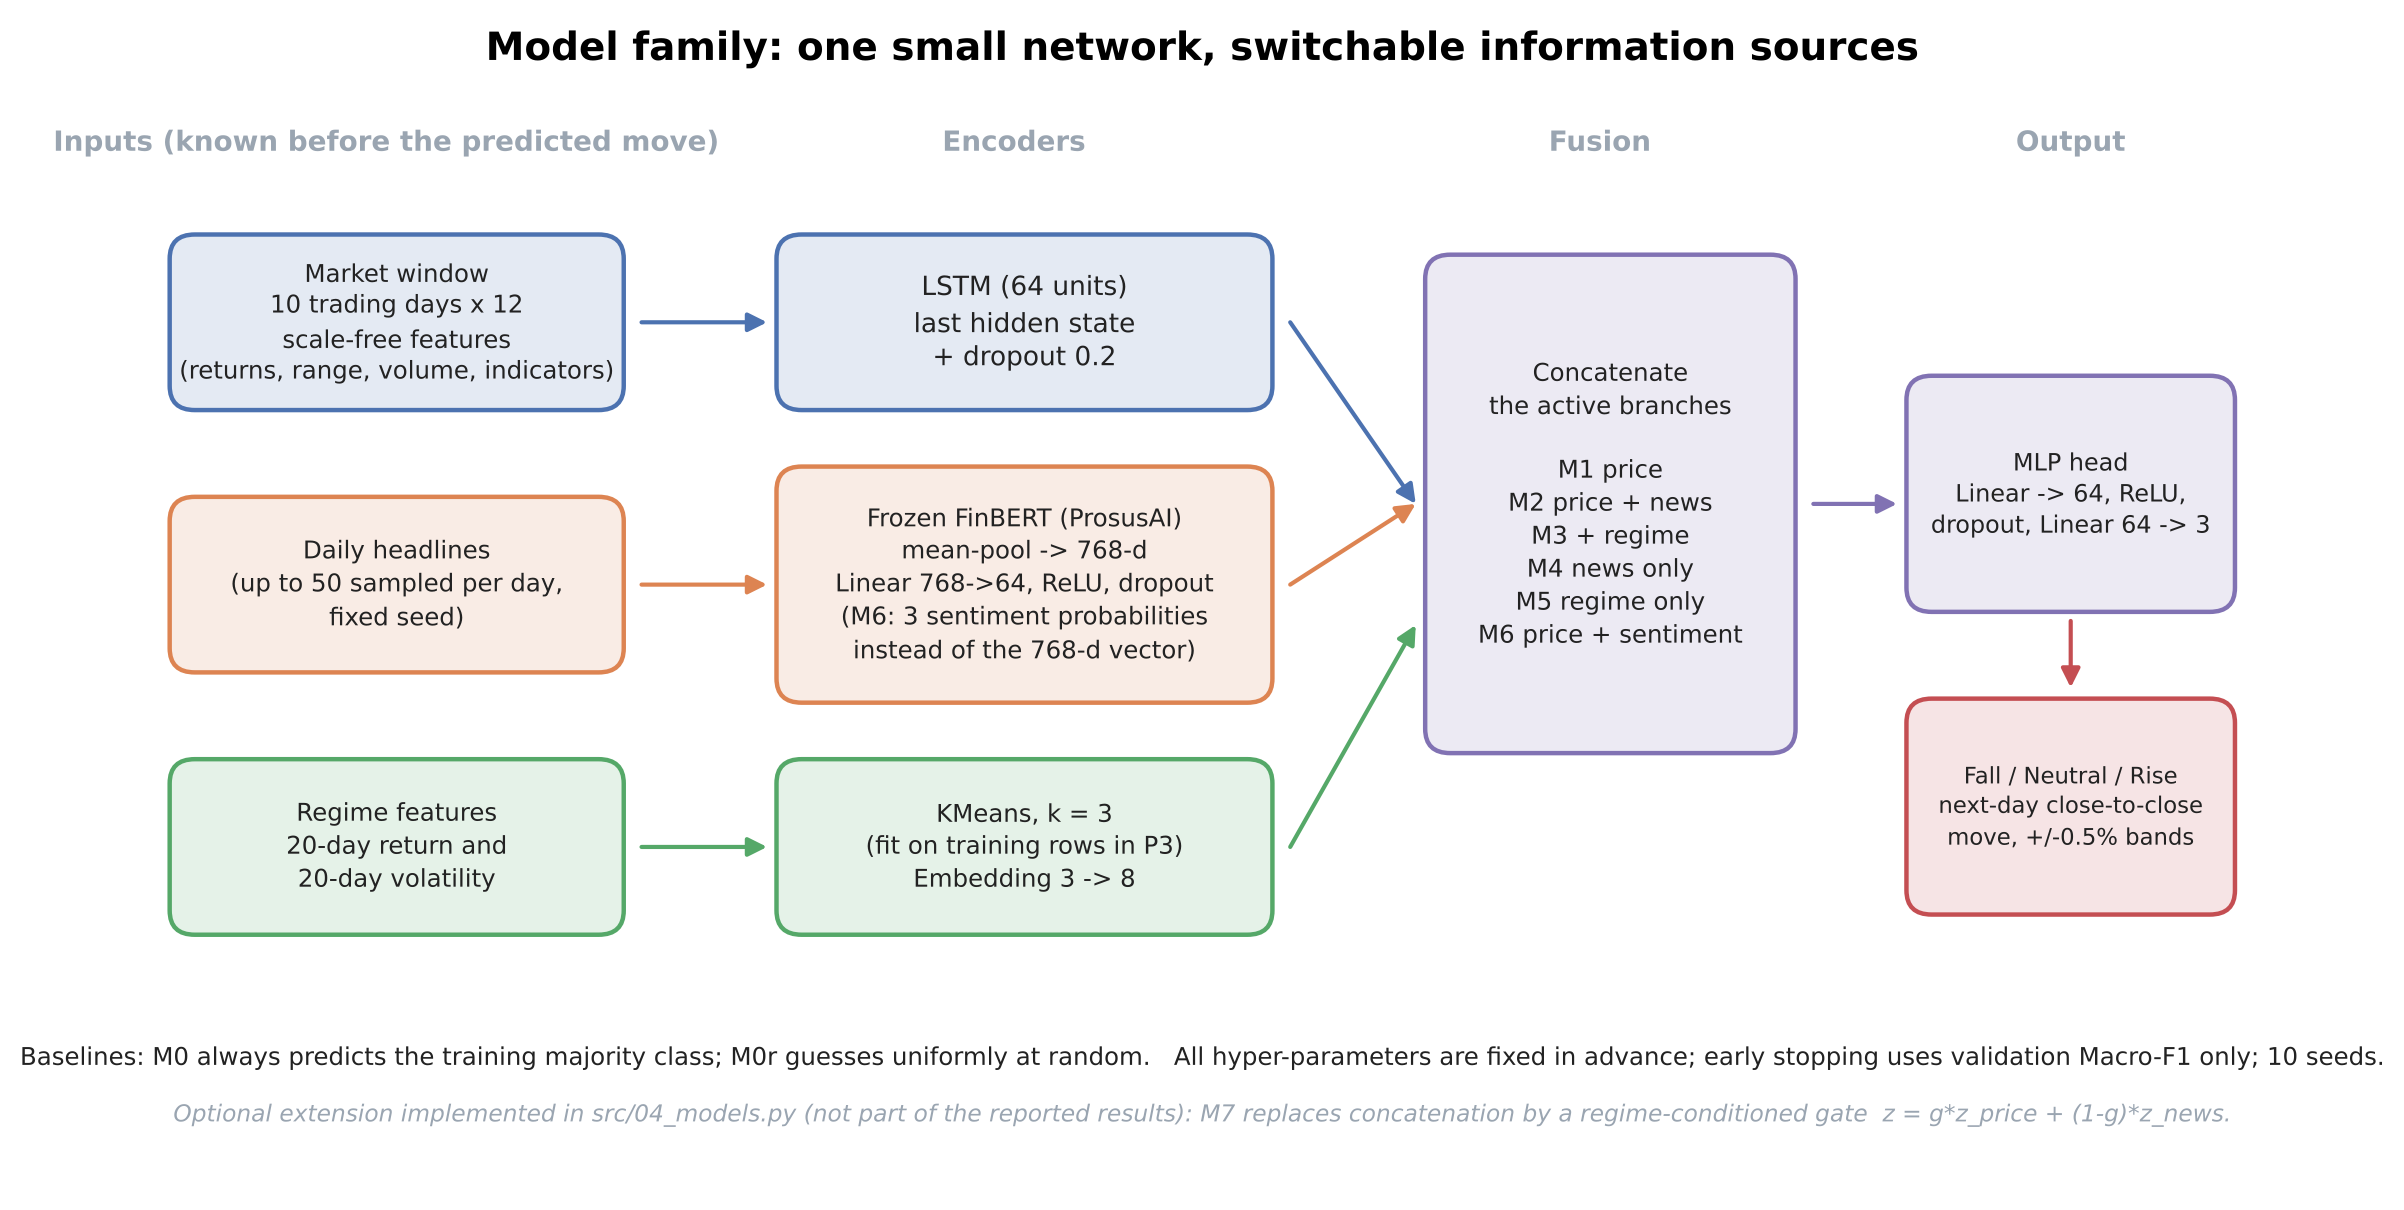
\includegraphics[width=0.96\textwidth]{fig_architecture.png}
\caption{Model family used in this report: one small network with switchable information sources.}
\end{figure}

\newpage
\tableofcontents
\clearpage
\addcontentsline{toc}{section}{List of Figures}
\listoffigures
\clearpage
\addcontentsline{toc}{section}{List of Tables}
\listoftables
\clearpage
\section{Introduction}
Predicting the direction of financial markets is one of the most studied applications of machine learning, and it is also one of the easiest in which to be misled. Reported accuracies depend not only on the model but on a long list of experimental choices: how the data are split, which statistics are used to scale the inputs, which regime of the market the test period happens to cover, and how many configurations were tried before the best was reported. At the same time, many recent studies add unstructured information, mainly news text encoded by pre-trained language models, to price-based networks and report improvements. Whether those improvements survive a strict evaluation, and whether they are uniform across calm and turbulent markets, is a more delicate question than a single headline number can answer.

This report treats the \textbf{evaluation protocol} as an experimental variable. Using one public benchmark, one small and fixed network family and ten random seeds, it measures (i) how much the apparent performance of the \emph{same} models changes when the evaluation becomes stricter, and (ii) whether financial news adds information beyond lagged prices, overall, within volatility regimes, and during the COVID-19 market stress of early 2020.

\begin{defbox}
\textbf{One-sentence summary.} On the NIFTY benchmark with strict chronological evaluation, a small price-only LSTM was the model to beat: FinBERT embeddings reduced out-of-sample Macro-F1, a three-number sentiment summary gave at most a small and statistically unreliable gain, and loosening the evaluation protocol did not systematically inflate scores.
\end{defbox}

\subsection{Motivation}
Three observations motivate the study.
\begin{itemize}
\item \textbf{Comparisons across papers are fragile.} Studies differ in assets, periods, label definitions, splits, metrics and preprocessing, so numbers are rarely comparable. Kraus and Feuerriegel \cite{kraus2017} make this point explicitly for text-based stock-reaction prediction.
\item \textbf{A single historical backtest is weak evidence.} Bailey et al.\ \cite{bailey2014,bailey2015} show formally that trying many configurations on one historical sample makes a strong in-sample result likely even when there is no skill. The practical remedy is to freeze the design in advance, report everything that was run and use strict out-of-time evaluation.
\item \textbf{The value of news may depend on the market state.} It is plausible, though not guaranteed, that headlines matter more when markets are stressed. This requires an explicit notion of market regime and a regime-wise evaluation.
\end{itemize}

\subsection{Research Questions}
\begin{keybox}
\textbf{RQ1 (evaluation sensitivity).} How much do reported results change when the same models are evaluated under increasingly strict temporal protocols (random split $\rightarrow$ chronological split $\rightarrow$ chronological split with train-only preprocessing)?\\[4pt]
\textbf{RQ2 (incremental value of news).} Does financial news provide predictive information beyond historical price data, and does its contribution vary across volatility regimes and during the February--April 2020 stress window?
\end{keybox}
Three testable hypotheses guide the analysis:
\begin{enumerate}[label=\textbf{H\arabic*:}]
\item Looser protocols overstate performance relative to the strict protocol.
\item The incremental value of news differs across market regimes.
\item An explicit regime input improves a price-plus-news model.
\end{enumerate}

\subsection{Contributions and Scope}
\begin{enumerate}
\item \textbf{A data audit of the NIFTY benchmark} (Chapter~\ref{ch:data}): the label is shown empirically to be the next trading day's close-to-close return; a daily price series of 2{,}695 trading days is recovered from overlapping contexts; the class mix and headline volume are shown to shift across the official splits.
\item \textbf{A controlled model family} (Chapter~\ref{ch:method}) in which each information source (price, news embedding, news sentiment, regime) can be switched on or off while architecture, optimiser and hyper-parameters stay fixed, together with a majority baseline and a uniform random-guess floor.
\item \textbf{A three-protocol leakage audit} with seed-level bootstrap intervals (Section~\ref{sec:protocol-results}).
\item \textbf{A regime-wise and stress-window analysis of news value} with row-level bootstrap intervals (Sections~\ref{sec:regime-results}--\ref{sec:stress}).
\item \textbf{A transparent record} of every post-hoc addition and of how many comparisons were examined (Appendix~\ref{app:transparency}).
\end{enumerate}
The study is deliberately small in architecture. It is \emph{not} an attempt to build a profitable trading strategy, it does not model transaction costs, and it claims nothing about causality or deployability.

\subsection{Report Organisation}
Chapter~\ref{ch:related} reviews background and related work. Chapter~\ref{ch:data} describes and audits the dataset. Chapter~\ref{ch:method} specifies features, regimes, models, training, protocols and statistics. Chapter~\ref{ch:results} reports results. Chapter~\ref{ch:discussion} interprets them and lists limitations, and Chapter~\ref{ch:conclusion} concludes. The appendices give the transparency statement and reproducibility details.

\newpage
\section{Background and Related Work}\label{ch:related}
\begin{infobox}
\textbf{Scope note.} This chapter summarises a deliberately small set of references whose bibliographic details were checked against arXiv, SSRN or publisher records. The descriptions of the individual papers are based on their abstracts and main claims; the chapter is a positioning of this study, not an exhaustive survey of the field.
\end{infobox}

\subsection{Sequence Models for Price-Based Forecasting}
Recurrent networks, and the Long Short-Term Memory (LSTM) cell in particular \cite{hochreiter1997}, are the standard building block for learning from windows of past market data. An LSTM reads a window of feature vectors one step at a time and keeps a gated memory; its final hidden state summarises the window and can be fed to a classifier. This report uses exactly that pattern with a small hidden size because the training set contains only about 1{,}460 labelled days.

\subsection{Financial News as an Input}
General language models are poorly calibrated to financial wording, so domain-adapted encoders are common. \textbf{FinBERT} \cite{araci2019} is a BERT model further pre-trained on financial text and fine-tuned for financial sentiment; it outputs a 768-dimensional representation and three class probabilities (positive, negative, neutral). Kraus and Feuerriegel \cite{kraus2017} studied deep networks with transfer learning to predict stock reactions from financial disclosures, and stress that results across studies are hard to compare because of differences in filtering, splits and metrics.

A line of recent work combines FinBERT-style sentiment with LSTM price models. Halder \cite{halder2022} reports a FinBERT-LSTM model on NASDAQ-100 stocks with New York Times articles; Gu et al.\ \cite{gu2024} use Benzinga news with a similar design; Karada\c{s} et al.\ \cite{karadas2025} combine tweets and news scored by large language models and FinBERT and report improvements of up to about five percent over an LSTM baseline. More elaborate fusion mechanisms include gated cross-attention for movement prediction \cite{zong2024} and confidence-calibrated late fusion across several equity indices and market regimes \cite{wang2026}. These works motivate the question of whether news helps, and they show that the field is moving towards complex fusion. This report keeps the architecture deliberately small and instead concentrates on evaluation.

\subsection{Evaluation Pitfalls in Financial Machine Learning}
Financial series are noisy, non-stationary and autocorrelated, which creates several risks.
\begin{itemize}
\item \textbf{Random splitting.} If overlapping windows from neighbouring days are shuffled across training and test sets, near-copies of test samples appear in training.
\item \textbf{Preprocessing leakage.} Scalers or clusters fitted on the full sample let test-period statistics shape the model inputs.
\item \textbf{Backtest overfitting.} Bailey et al.\ \cite{bailey2014,bailey2015} show that selecting the best of many configurations on one historical sample inflates apparent performance, and recommend disclosing the number of trials.
\end{itemize}
Chapter~\ref{ch:method} turns the first two risks into an explicit three-protocol experiment, and the third into the freezing of hyper-parameters and a full disclosure of every comparison made.

\subsection{Market Regimes}
Financial markets alternate between calm and turbulent phases. A regime is a persistent state of the market summarised here by recent return and volatility. Regime information can enter a model as an extra input, as a conditioning signal for fusion weights, or as a stratification variable for evaluation. This report uses regimes in the first and third ways: as an input (model M3) and as a way to ask whether news value differs between calm and turbulent days.

\subsection{Dataset: NIFTY}
The NIFTY dataset of Saqur et al.\ \cite{saqur2024} pairs daily market context for the SPY exchange-traded fund with curated news headlines and a Rise/Neutral/Fall label, and provides an official chronological train/validation/test split. Because it is public, it allows the experiments here to be reproduced exactly.

\subsection{Positioning}
\begin{keybox}
Prior work shows that financial news and multimodal models can help market prediction, while financial-ML research separately documents backtest overfitting and inconsistent evaluation. This report examines, within one controlled pipeline on a public benchmark, how much reported performance changes with the evaluation protocol, and whether the incremental value of news differs across volatility regimes, including the February--April 2020 stress period.
\end{keybox}
This is a statement of what this study does, not a claim to be the first to examine these questions; the reference list is short and a broader search may find closer work.

\newpage
\section{Data and Data Audit}\label{ch:data}
\subsection{The NIFTY Benchmark}
The experiments use the NIFTY dataset \cite{saqur2024} (Hugging Face identifier \texttt{raeidsaqur/NIFTY}). The market target is the SPY exchange-traded fund. The dataset contains 2{,}111 rows with the official chronological split of Table~\ref{tab:splits}. Each row provides a text prompt containing a short history of daily market statistics (open, high, low, close, adjusted close, volume, percentage change and several technical indicators), a block of news headlines, a categorical label (Fall, Neutral or Rise) and a numeric \texttt{pct\_change}. The label rule is: Fall if the change is below $-0.5\%$, Rise if it is above $+0.5\%$, and Neutral otherwise.

\begin{table}[H]
\centering
\begin{tabular}{lrrrr}
\toprule
Split & Rows (raw) & Rows (used) & First date & Last date\\
\midrule
Train & 1{,}477 & 1{,}462 & 2010-01-06$^{*}$ & 2017-06-27\\
Validation & 317 & 317 & 2017-06-28 & 2019-02-12\\
Test & 317 & 317 & 2019-02-13 & 2020-09-21\\
\midrule
Total & 2{,}111 & 2{,}096 & & \\
\bottomrule
\end{tabular}
\caption[Official NIFTY splits and rows used]{Official NIFTY splits. Fifteen early training rows are dropped because the 20-day regime features need 20 days of history (Section~\ref{sec:windows}). $^{*}$First date of the raw rows; the dropped rows span 2010-01-06 to 2010-02-02, so the first row used is later.}\label{tab:splits}
\end{table}
\figpage{fig_dataset_timeline.png}{\textwidth}{Official chronological split and the stress-period case study window.}

\subsection{The Label Is the Next Trading Day's Return}
A first check established what the label actually measures, because the timing convention determines what may legitimately be used as an input. For each row, the \texttt{pct\_change} target was compared with several candidate returns computed from the market data embedded in the contexts. The result on 2{,}110 rows with a defined next day was unambiguous:
\begin{center}
\begin{tabular}{lc}
\toprule
Candidate series & Share within $10^{-3}$ of the target\\
\midrule
Next-day close-to-close return & \textbf{1.000}\\
Same-day close-to-close return & 0.066\\
Previous-day close-to-close return & 0.081\\
Same-day open-to-close return & 0.087\\
Context \texttt{pct\_change} of the same date & 0.064\\
\bottomrule
\end{tabular}
\end{center}
\begin{defbox}
\textbf{Timing convention.} The label of a row dated $t$ is the close-to-close return from day $t$ to the next trading day $t{+}1$. A price window may therefore end at day $t$ (the most recent information available before the predicted move). This is called $\mathrm{LAG}=0$ in the code. The benchmark's own prompt uses a window ending at $t{-}1$; this alternative ($\mathrm{LAG}=1$) is implemented as a robustness option but was not run for this report.
\end{defbox}
Ten of the 2{,}111 rows lie exactly on the $\pm0.5\%$ boundary and disagree with the label rule, most likely through rounding of \texttt{pct\_change} to four decimals (the unrounded values were not inspected; for example 2012-06-14 and 2017-11-14); they were kept. The 2{,}110 valid comparisons exclude one row, the final test date 2020-09-21, whose next trading day lies beyond the recovered series.

\subsection{Recovering a Daily Price Series}\label{sec:windows}
The dataset is not a daily series: target dates are separated by one to four business days (1{,}544 consecutive pairs, 469 gaps of two, 77 of three and 20 of four), and there are 2{,}111 rows against about 2{,}700 NYSE trading days in the same range. However, every row carries several trading days of market context (context lengths 1--8 days, 5--8 for almost all rows), and consecutive contexts overlap. Merging all contexts yields \textbf{2{,}695 distinct trading days} from 2010-01-05 to 2020-09-18. Where the same day appears in several contexts the values agree exactly (maximum disagreement in close: 0.0). Checked against the NYSE calendar, the recovered series contains every session in this range except one (2018-12-31), which is not interpolated. The fourteen other dates flagged by the first audit (Good Fridays, 2012-10-29/30 and 2018-12-05) are market closures, not missing data.

Price windows are then built from this daily series, so a ``10-day'' window means ten consecutive \emph{trading} days (the maximum calendar span of a window is 18 days), not ten rows of the sparse dataset. A window for a row dated $t$ ends at the last recovered trading day not after $t$. Because 20 days of history are needed for the regime features, the 15 earliest rows are dropped, leaving 1{,}462, 317 and 317 rows (Table~\ref{tab:splits}).

\begin{warnbox}
\textbf{Leakage guards.} The code asserts for every window and for every regime feature that its last day is not after the row's date, and that all P2/P3 splits are chronological. A further check confirms that the first column of each window equals the raw close-to-close return stored by the first processing step.
\end{warnbox}

\subsection{Class Balance Shifts Across Splits}
Table~\ref{tab:classes} shows that the label mix is not stable. The Neutral share is 53.5\% in training but 45.1\% in the test period, which contains the 2020 shock.
\begin{table}[H]
\centering
\begin{tabular}{lccc}
\toprule
Split & Fall & Neutral & Rise\\
\midrule
Train & 0.205 & 0.535 & 0.260\\
Validation & 0.167 & 0.596 & 0.237\\
Test & 0.230 & 0.451 & 0.319\\
\bottomrule
\end{tabular}
\caption{Label shares by official split.}\label{tab:classes}
\end{table}
Always predicting the training majority class (Neutral) therefore reaches an accuracy of 0.451 on the test set but a Macro-F1 of only $0.207$, because two of the three classes get an F1 of zero. For this reason Macro-F1 is the primary metric and a \emph{uniform random guesser} (Macro-F1 $\approx0.333$) is used as the meaningful floor.

\subsection{News Headlines}
Each row carries a block of daily headlines (mean about 207 headlines per row in the raw text over all 2{,}111 rows, with the number depending strongly on the era). Over the 2{,}096 modelling rows the raw volume falls sharply across the splits: the mean number of headlines per day is about 277 in the training period (maximum 1{,}627), 54 in validation and 26 in test. To bound compute and reduce this imbalance, at most 50 headlines per day are sampled at random (fixed seed 1234) before encoding; after this cap the mean is 49.0 (train), 46.4 (validation) and 26.2 (test) headlines per day. Across all splits 94{,}652 headlines were embedded and no day was left without a headline.

Mean FinBERT sentiment (probability of positive minus probability of negative) also moves across periods: $-0.068$ in training, $-0.095$ in validation and $-0.184$ in test, and in March 2020 alone it falls to $-0.319$ against $-0.176$ for the rest of the test set. As a diagnostic of how much information the daily embedding carries, the average cosine similarity (ratio of the mean dot product to the product of mean norms) between embeddings of consecutive dataset rows is 0.963, against 0.951 for random pairs of days, so the mean-pooled embedding varies only slightly from day to day. These shifts in news volume and tone are a confound for any news result and are returned to in Chapter~\ref{ch:discussion}.

\subsection{Exploratory Overview}
\figpage{eda_overview.png}{\textwidth}{Exploratory overview of the benchmark (price history, label mix and news volume by split).}

\newpage
\section{Methodology}\label{ch:method}
\subsection{Problem Definition}
For each row dated $t$ the task is three-class classification of the next trading day's return $r_{t\to t+1}$ into $y_t\in\{\text{Fall},\text{Neutral},\text{Rise}\}$. The inputs available are a window $X_t\in\mathbb{R}^{10\times12}$ of price features ending at $t$, a news representation $n_t$ built from the headlines dated $t$, and a regime label $g_t\in\{\text{Low-vol},\text{Mid-vol},\text{High-vol}\}$. The primary metric is Macro-F1,
\[
\mathrm{Macro\text{-}}\Fone=\frac13\sum_{c\in\{\text{Fall},\text{Neutral},\text{Rise}\}}\Fone^{(c)},\qquad
\Fone^{(c)}=\frac{2\,P_cR_c}{P_c+R_c},
\]
with accuracy and balanced accuracy (mean per-class recall) reported alongside.

\subsection{Price Features}
Raw price levels drift from about 100 to 340 over the sample, so test-period inputs would sit far outside the training range. Twelve \emph{scale-free} features are therefore computed from the recovered daily series (Table~\ref{tab:features}).
\begin{table}[H]
\centering
\begin{tabular}{ll}
\toprule
Name & Definition\\
\midrule
\texttt{ret} & daily close-to-close return\\
\texttt{oc} & close/open $-1$\\
\texttt{hl} & (high $-$ low)/close\\
\texttt{lvol\_rel} & log volume minus its trailing 20-day mean\\
\texttt{macd\_n} & MACD/close\\
\texttt{rsi}, \texttt{cci}, \texttt{dx} & 30-day RSI, CCI and DX, each divided by 100\\
\texttt{bollpos} & (close $-$ lower band)/(upper $-$ lower band)\\
\texttt{bollw} & (upper $-$ lower band)/close\\
\texttt{c\_sma30}, \texttt{c\_sma60} & close/30-day (60-day) simple moving average $-1$\\
\bottomrule
\end{tabular}
\caption{The 12 scale-free price features. Indicator columns (MACD, RSI, CCI, DX, Bollinger bands, moving averages) are those supplied by the dataset.}\label{tab:features}
\end{table}
Features are standardised with a mean and standard deviation estimated on the rows allowed by the protocol (Section~\ref{sec:protocols}) and clipped to $\pm5$ standard deviations to limit the effect of extreme 2020 values.

\subsection{News Representation}
Headlines of day $t$ are encoded by the frozen \texttt{ProsusAI/finbert} model \cite{araci2019} (maximum 64 tokens per headline, batch size 256). Up to 50 headlines per day are sampled with a fixed seed. Two representations are produced per day:
\begin{enumerate}
\item the \textbf{embedding}: the mean of the 768-dimensional headline representations; and
\item the \textbf{sentiment}: the mean of the three FinBERT class probabilities (positive, negative, neutral).
\end{enumerate}
FinBERT is never fine-tuned; all learning on the news side happens in a small downstream layer.

\subsection{Market Regimes}
Two regime features use only prices up to the row's date: the 20-day return $\mathrm{ret}_{20}=C_t/C_{t-20}-1$ and the log of the 20-day standard deviation of daily returns, $\log\sigma_{20}$. The logarithm is used because volatility is right-skewed, so that clusters are not dominated by a few crashes. After standardisation, \textbf{$k$-means with $k=3$} (ten initialisations, fixed seed) assigns each day to a cluster. Clusters are named \emph{Low-vol}, \emph{Mid-vol} and \emph{High-vol} purely by ranking their mean log-volatility; no economic meaning beyond that ranking is assumed.

For the strict protocol the scaler and clustering are fitted on training rows only; for the looser protocols they are fitted on all rows. The two assignments agree on 93.6\% of rows (92.3\% in train, 98.1\% in validation, 94.9\% in test).

\begin{table}[H]
\centering
\begin{tabular}{lrrrrr}
\toprule
Regime & $n$ (train) & mean $\mathrm{ret}_{20}$ & mean $\sigma_{20}$ & mean next-day ret. & share\\
\midrule
Low-vol & 700 & 0.0185 & 0.0055 & $-0.0000$ & 0.479\\
Mid-vol & 411 & 0.0319 & 0.0103 & 0.0009 & 0.281\\
High-vol & 351 & $-0.0363$ & 0.0126 & 0.0010 & 0.240\\
\bottomrule
\end{tabular}
\caption{Regime statistics on training rows (strict-protocol fit).}\label{tab:regimestats}
\end{table}
Regimes persist (Table~\ref{tab:transition}): the daily probability of staying in Low-vol is 0.961, and the median run length is 15 trading days for Low-vol but only 4 for Mid-vol and High-vol, so the intermediate and high regimes switch frequently. The regime mix also changes across splits: High-vol accounts for 24\% of rows in train, 24\% in validation and 25\% in test, whereas Low-vol falls from 64\% in validation to 39\% in test.
\begin{table}[H]
\centering
\begin{tabular}{lccc}
\toprule
From $\backslash$ To & Low-vol & Mid-vol & High-vol\\
\midrule
Low-vol & 0.961 & 0.017 & 0.021\\
Mid-vol & 0.058 & 0.869 & 0.073\\
High-vol & 0.016 & 0.109 & 0.875\\
\bottomrule
\end{tabular}
\caption{Daily regime transition matrix (strict-protocol model).}\label{tab:transition}
\end{table}
\figpage{regimes_overview.png}{\textwidth}{Left: SPY close coloured by regime (strict fit); dashed lines mark the validation and test starts. Right: training rows in regime-feature space with the three cluster centres.}

Across all rows, the label mix differs strongly by regime: the share of Neutral next days is 64.2\% in Low-vol, 54.9\% in Mid-vol and only 28.8\% in High-vol, where Rise (40.6\%) and Fall (30.6\%) dominate. Regimes therefore carry information about the \emph{size} of the next move rather than its sign.

\subsection{Model Family}
All learned models share one architecture whose branches are switched on or off (Figure~1 in the abstract; Table~\ref{tab:models}).
\begin{table}[H]
\centering
\begin{tabular}{llp{6.6cm}}
\toprule
Model & Inputs & Purpose\\
\midrule
M0 & training majority class & deterministic baseline\\
M0r & uniform random guess & chance floor for Macro-F1\\
M1 & price window & price-only benchmark\\
M2 & price + FinBERT embedding & multimodal benchmark\\
M3 & price + embedding + regime & regime-aware multimodal model\\
M4 & embedding only & news-only ablation\\
M5 & regime only & regime-only ablation\\
M6 & price + 3 sentiment scores & compact news-fusion model (added post hoc)\\
\bottomrule
\end{tabular}
\caption{Model family.}\label{tab:models}
\end{table}
The branches are: an \textbf{LSTM} \cite{hochreiter1997} with 64 hidden units whose last hidden state (with dropout 0.2) summarises the price window; a \textbf{news branch} that maps the news vector (768 dimensions for the embedding, 3 for the sentiment) through a linear layer to 64 units with ReLU and dropout; and a \textbf{regime branch}, an embedding of the three regime ids into 8 dimensions. Active branch outputs are concatenated and passed to a head of Linear$(\cdot\to64)$, ReLU, dropout, Linear$(64\to3)$ with softmax cross-entropy.

An additional gated variant (M7), in which a regime-conditioned gate $g=\sigma(W[z_{\text{price}};z_{\text{news}};e_{\text{regime}}])$ mixes the price and news embeddings as $z=g\odot z_{\text{price}}+(1-g)\odot z_{\text{news}}$, is implemented in the code repository. M7 was \emph{not} run on the real data and is not part of the reported results; it is left as future work (Chapter~\ref{ch:conclusion}).

\subsection{Training Procedure}
\begin{defbox}
\textbf{Frozen settings (never tuned on the test set).} Adam optimiser, learning rate $10^{-3}$, weight decay $10^{-4}$, batch size 64, at most 50 epochs, early stopping with patience 8 on \emph{validation} Macro-F1, class-weighted cross-entropy (weights inversely proportional to training class counts), input clipping at $\pm5$ standard deviations. LSTM hidden size 64, dropout 0.2, news output 64, regime embedding 8. Ten seeds (0--9).
\end{defbox}
Hyper-parameters were chosen once, before the main experiments, from conventional values and were not searched. The checkpoint with the best validation Macro-F1 is used for the reported test predictions. The random guesser M0r draws labels uniformly at random with the run's seed.

\subsection{Evaluation Protocols}\label{sec:protocols}
The same models are evaluated under three protocols (Figure~\ref{fig:protocols}) that differ in how data are split and which rows are used to fit preprocessing and regimes.
\begin{table}[H]
\centering
\begin{tabular}{llll}
\toprule
Protocol & Split & Scalers fitted on & Regimes fitted on\\
\midrule
P1 & random (same sizes) & all rows & all rows\\
P2 & chronological & all rows & all rows\\
P3 (primary) & chronological & train rows only & train rows only\\
\bottomrule
\end{tabular}
\caption{Evaluation protocols.}
\end{table}
P1 is deliberately invalid and serves as a permissive reference; P3 is the primary benchmark for all scientific conclusions. In P1 a different random split is drawn for each seed with the same train/validation/test sizes, so the P1 test sample differs from the P2/P3 test sample; the gaps between protocols therefore mix leakage and sampling effects (Chapter~\ref{ch:discussion}).
\begin{figure}[H]
\centering
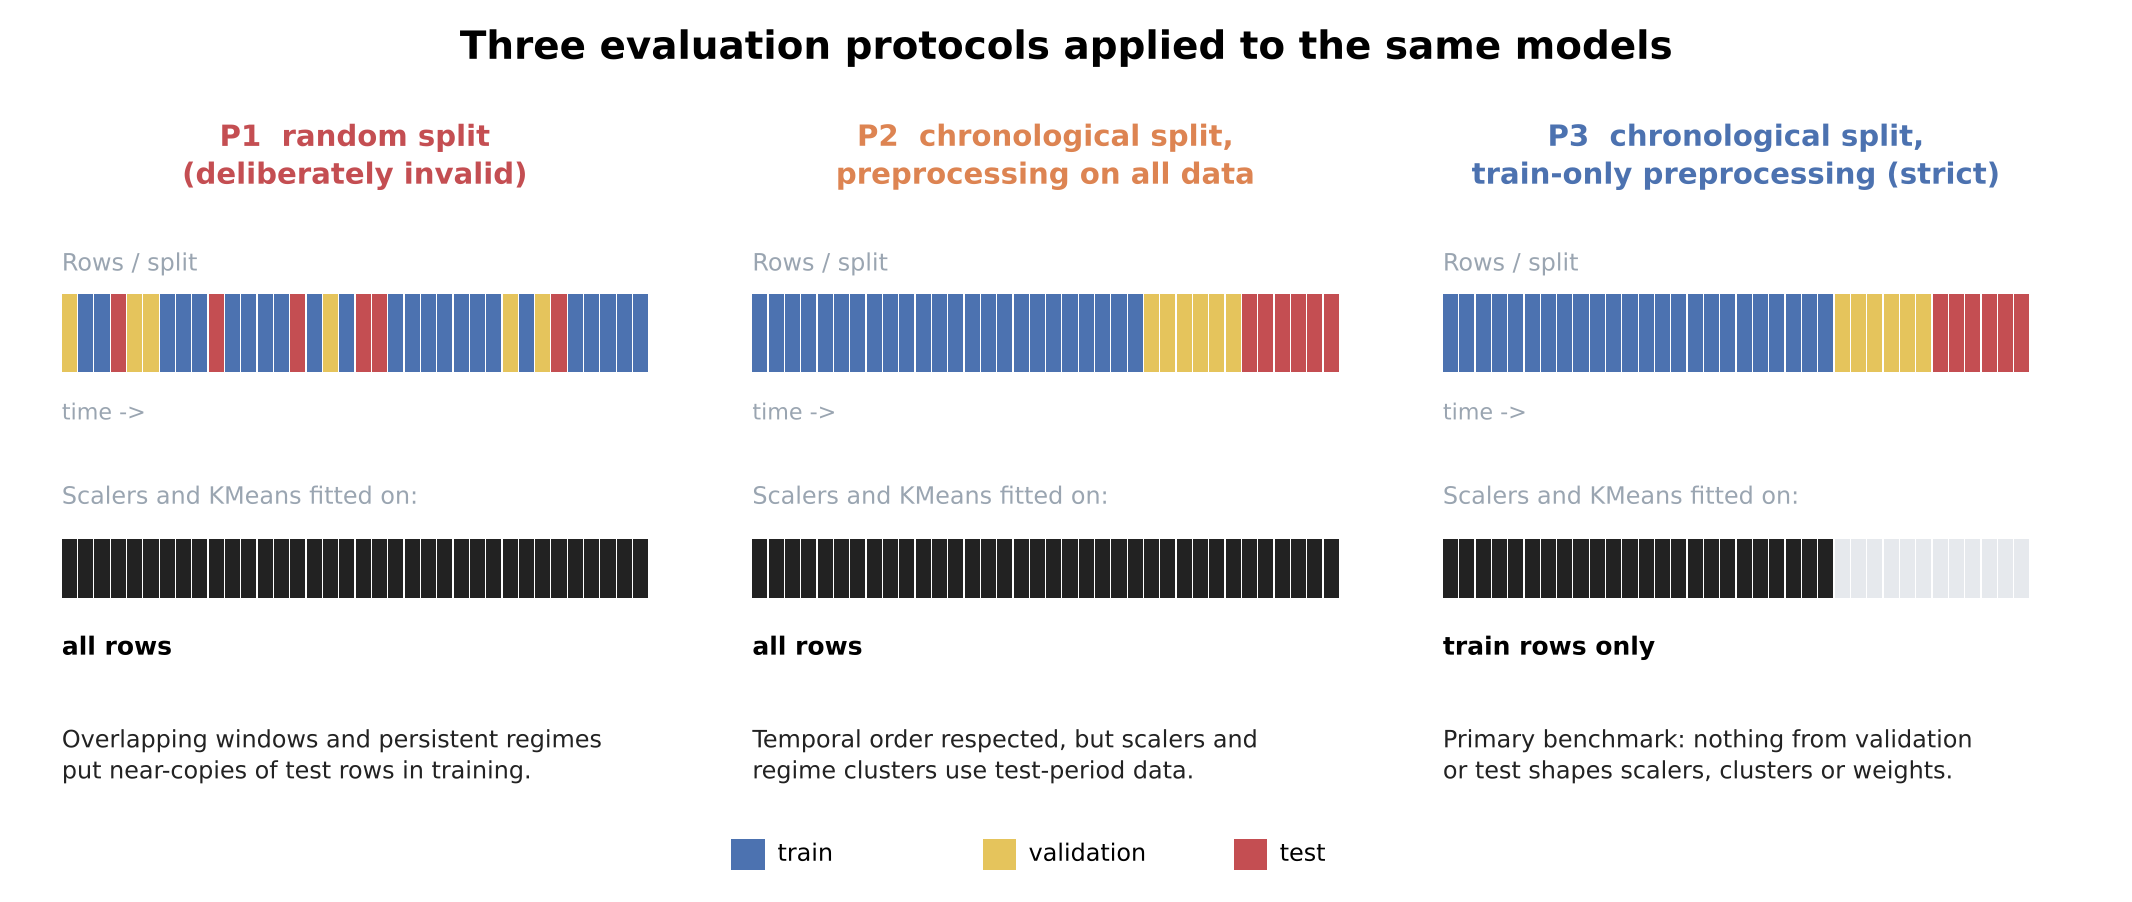
\includegraphics[width=\textwidth]{fig_protocol_design.png}
\caption{The three evaluation protocols. Dark squares in the lower strip mark the rows used to fit scalers and regime clusters.}\label{fig:protocols}
\end{figure}

\subsection{Statistical Inference}
\paragraph{Protocol gaps (RQ1).} For each model the gap is the difference between the mean test Macro-F1 under a looser protocol and under P3. A 95\% interval is obtained by bootstrapping the 10 per-seed scores of each protocol separately (1{,}000 resamples).
\paragraph{News value (RQ2).} For each group (all test rows, each regime, the stress window, and its complement), the seed-averaged predictions of each model are evaluated on test rows resampled with replacement (1{,}000 draws, the same resample for every model), and the difference in Macro-F1 between two models is computed on each resample. The 2.5th and 97.5th percentiles give the interval. These intervals describe test-set sampling uncertainty.
\paragraph{Stress window.} The stress window is 1 February to 30 April 2020 and contains 50 test rows; the regime groups contain 125 (Low-vol), 113 (Mid-vol) and 79 (High-vol) test rows.
\paragraph{Multiplicity.} About 24 pairwise comparisons are reported; an isolated interval that excludes zero is therefore treated as a hypothesis, not as a finding.

\subsection{Implementation}
All code is in Python with PyTorch, scikit-learn, pandas and the Hugging Face \texttt{transformers} library, and is available in the accompanying repository. FinBERT embedding was run on a GPU; models were trained on CPU in Google Colab. Training all models under all three protocols for ten seeds (270 runs) takes a few minutes on a CPU.

\newpage
\section{Results}\label{ch:results}
\subsection{Reporting Conventions}
All numbers are means over ten seeds unless stated otherwise. Tables report test Macro-F1 under the strict protocol P3 unless a different protocol is named. The test set has 317 rows. M0 always predicts the training majority class; M0r guesses uniformly at random and is the appropriate floor for Macro-F1. Every value below is taken from the executed ten-seed run; no hyper-parameter was changed after the pilot run (pilot outputs were not saved, so this cannot be independently verified); M0r and M6 were added after the pilot.

\subsection{Overall Comparison Under the Strict Protocol}\label{sec:overall}
\begin{table}[H]
\centering
\begin{tabular}{llcccc}
\toprule
Model & Inputs & Macro-F1 & Accuracy & Balanced acc.\\
\midrule
M0 & majority class & 0.207 $\pm$ 0.000 & 0.451 & 0.333\\
M0r & uniform random guess & 0.333 $\pm$ 0.020 & 0.339 & 0.341\\
M1 & price window & \textbf{0.466} $\pm$ 0.036 & 0.530 & 0.476\\
M2 & price + FinBERT embedding & 0.416 $\pm$ 0.023 & 0.493 & 0.448\\
M3 & price + embedding + regime & 0.433 $\pm$ 0.025 & 0.491 & 0.454\\
M4 & embedding only & 0.382 $\pm$ 0.037 & 0.402 & 0.394\\
M5 & regime only & 0.354 $\pm$ 0.019 & 0.493 & 0.415\\
M6 & price + sentiment (3 scores) & \textbf{0.482} $\pm$ 0.038 & 0.531 & 0.498\\
\bottomrule
\end{tabular}
\caption[Test performance under the strict protocol P3]{Test performance under the strict protocol P3 (Macro-F1 mean $\pm$ s.d.\ over 10 seeds). M1 and M6 are not reliably different (Table~\ref{tab:diffs}).}\label{tab:main}
\end{table}
All learned models exceed the random-guess floor. The price-only model is competitive with every richer model, the news-only model reaches 0.382, and the regime-only model is close to the floor in Macro-F1 although its accuracy (0.493) is similar to that of the richer models, which shows why accuracy alone is a poor guide on this data.

\begin{table}[H]
\centering
\begin{tabular}{lcccc}
\toprule
Model & Train Macro-F1 & Valid Macro-F1 & Test Macro-F1 & Train $-$ Test\\
\midrule
M0 & 0.232 & 0.249 & 0.207 & 0.025\\
M0r & 0.315 & 0.291 & 0.333 & $-$0.018\\
M1 & 0.477 & 0.464 & 0.466 & 0.011\\
M2 & 0.554 & 0.452 & 0.416 & 0.138\\
M3 & 0.569 & 0.461 & 0.433 & 0.136\\
M4 & 0.701 & 0.378 & 0.382 & 0.319\\
M5 & 0.360 & 0.390 & 0.354 & 0.006\\
M6 & 0.486 & 0.456 & 0.482 & 0.004\\
\bottomrule
\end{tabular}
\caption[Train, validation and test Macro-F1 under P3 (table)]{Macro-F1 on training, validation and test rows under P3 (mean over 10 seeds). Large train--test gaps for the models using the 768-dimensional embedding (M2, M3, M4) indicate overfitting.}\label{tab:overfit}
\end{table}
Table~\ref{tab:overfit} shows that the price-only model has almost no train--test gap (0.477 versus 0.466), whereas adding the 768-dimensional embedding raises training Macro-F1 to 0.554 and lowers test Macro-F1 to 0.416. The news-only model fits training rows well (0.701) but generalises poorly (0.382). Figure~\ref{fig:tvt} shows the same numbers: for M2, M3 and M4 the training bar sits well above the validation and test bars, whereas for M1 and M6 the three bars are close.
\begin{figure}[H]\centering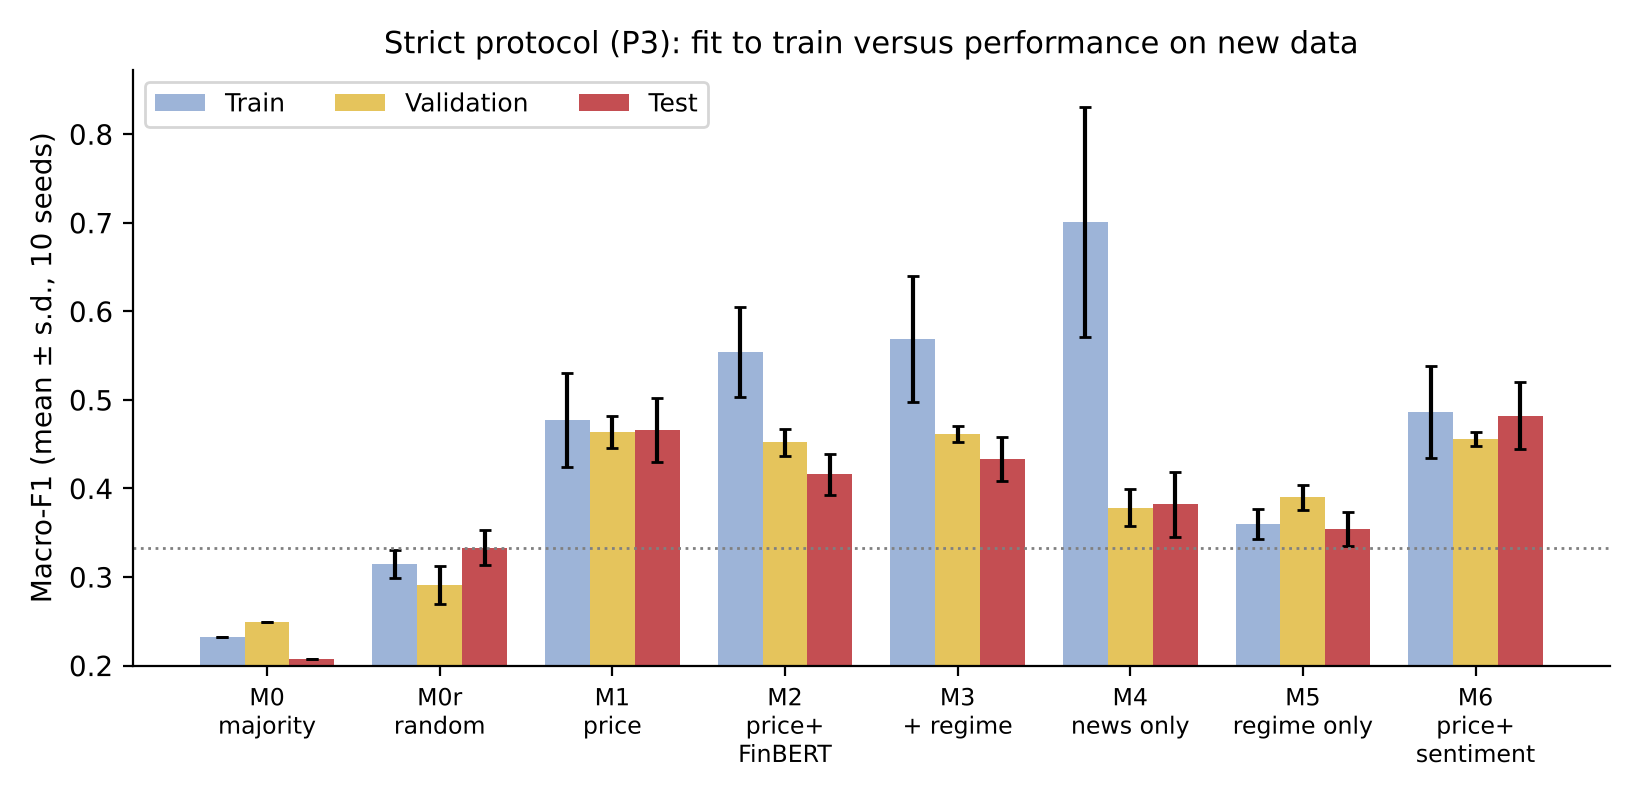
\includegraphics[width=\textwidth]{fig_train_valid_test.png}\caption[Train, validation and test Macro-F1 under P3 (figure)]{Macro-F1 on training, validation and test rows under P3 (mean $\pm$ s.d.\ over ten seeds; dotted line: random-guess level 0.333). Same values as Table~\ref{tab:overfit}.}\label{fig:tvt}\end{figure}

\subsection{Effect of the Evaluation Protocol (RQ1)}\label{sec:protocol-results}
\begin{table}[H]
\centering
\begin{tabular}{lccc}
\toprule
Model & P1 random, fit all & P2 chronological, fit all & P3 strict\\
\midrule
M0 & 0.228 & 0.207 & 0.207\\
M0r & 0.315 & 0.333 & 0.333\\
M1 price & 0.438 & 0.460 & 0.466\\
M2 price + embedding & 0.423 & 0.428 & 0.416\\
M3 price + emb.\ + regime & 0.421 & 0.441 & 0.433\\
M4 embedding only & 0.363 & 0.369 & 0.382\\
M5 regime only & 0.400 & 0.382 & 0.354\\
M6 price + sentiment & 0.431 & 0.448 & 0.482\\
\bottomrule
\end{tabular}
\caption{Test Macro-F1 by protocol (mean over 10 seeds).}
\end{table}
\begin{table}[H]
\centering
\begin{tabular}{lcc}
\toprule
Model & P1 $-$ P3 & P2 $-$ P3\\
\midrule
M1 & $-0.028$ [$-0.055$, 0.001] & $-0.005$ [$-0.034$, 0.023]\\
M2 & $+0.006$ [$-0.010$, 0.022] & $+0.012$ [$-0.008$, 0.031]\\
M3 & $-0.012$ [$-0.030$, 0.008] & $+0.008$ [$-0.010$, 0.028]\\
M4 & $-0.019$ [$-0.040$, 0.004] & $-0.013$ [$-0.043$, 0.018]\\
M5 & \textbf{$+0.046$ [0.029, 0.063]} & \textbf{$+0.028$ [0.007, 0.048]}\\
M6 & \textbf{$-0.051$ [$-0.079$, $-0.019$]} & $-0.034$ [$-0.071$, 0.005]\\
\bottomrule
\end{tabular}
\caption[Protocol gaps (looser protocol minus P3) with 95\% intervals]{Optimistic performance gap (looser protocol minus P3) with 95\% bootstrap intervals over seeds. Positive values mean the looser protocol scores higher. Intervals resample the ten seeds of each protocol independently; they exclude test-row uncertainty, and P1 also changes the test sample.}\label{tab:gaps}
\end{table}
\begin{figure}[H]\centering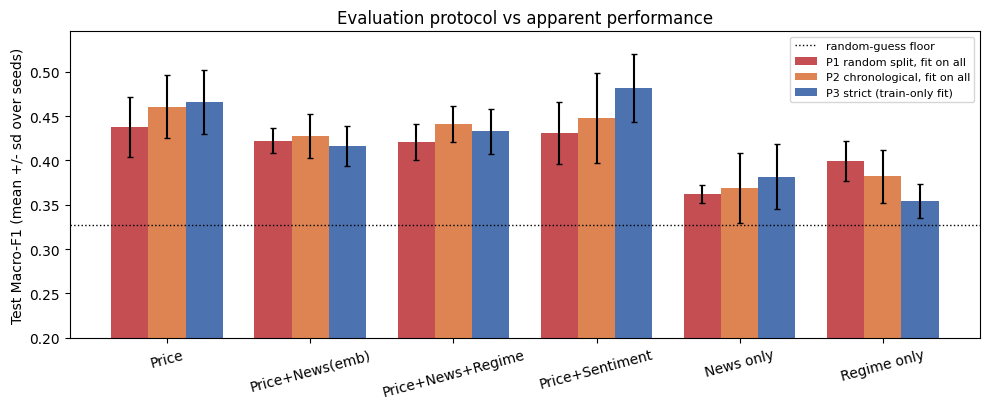
\includegraphics[width=\textwidth]{fig_protocol_audit.png}\caption[Test Macro-F1 under the three evaluation protocols]{Test Macro-F1 under the three evaluation protocols (mean over ten seeds, error bars $\pm1$ s.d.; dotted line: mean random-guess score, about 0.33). The protocol gaps are in Table~\ref{tab:gaps}.}\end{figure}
Figure~\ref{fig:seeds} plots every one of the 240 evaluations behind these bars. For the trained models the standard deviation over the ten seeds is between 0.010 and 0.051 depending on model and protocol (0.019 to 0.038 under P3, Table~\ref{tab:main}), which is as large as many of the differences between models and protocols; this is why intervals, rather than point differences, are used throughout. The majority-class baseline M0 has almost no spread under P2 and P3 because it is deterministic, and the regime-only model M5 repeats a few values, as expected for an input that takes only three distinct values.
\begin{figure}[H]\centering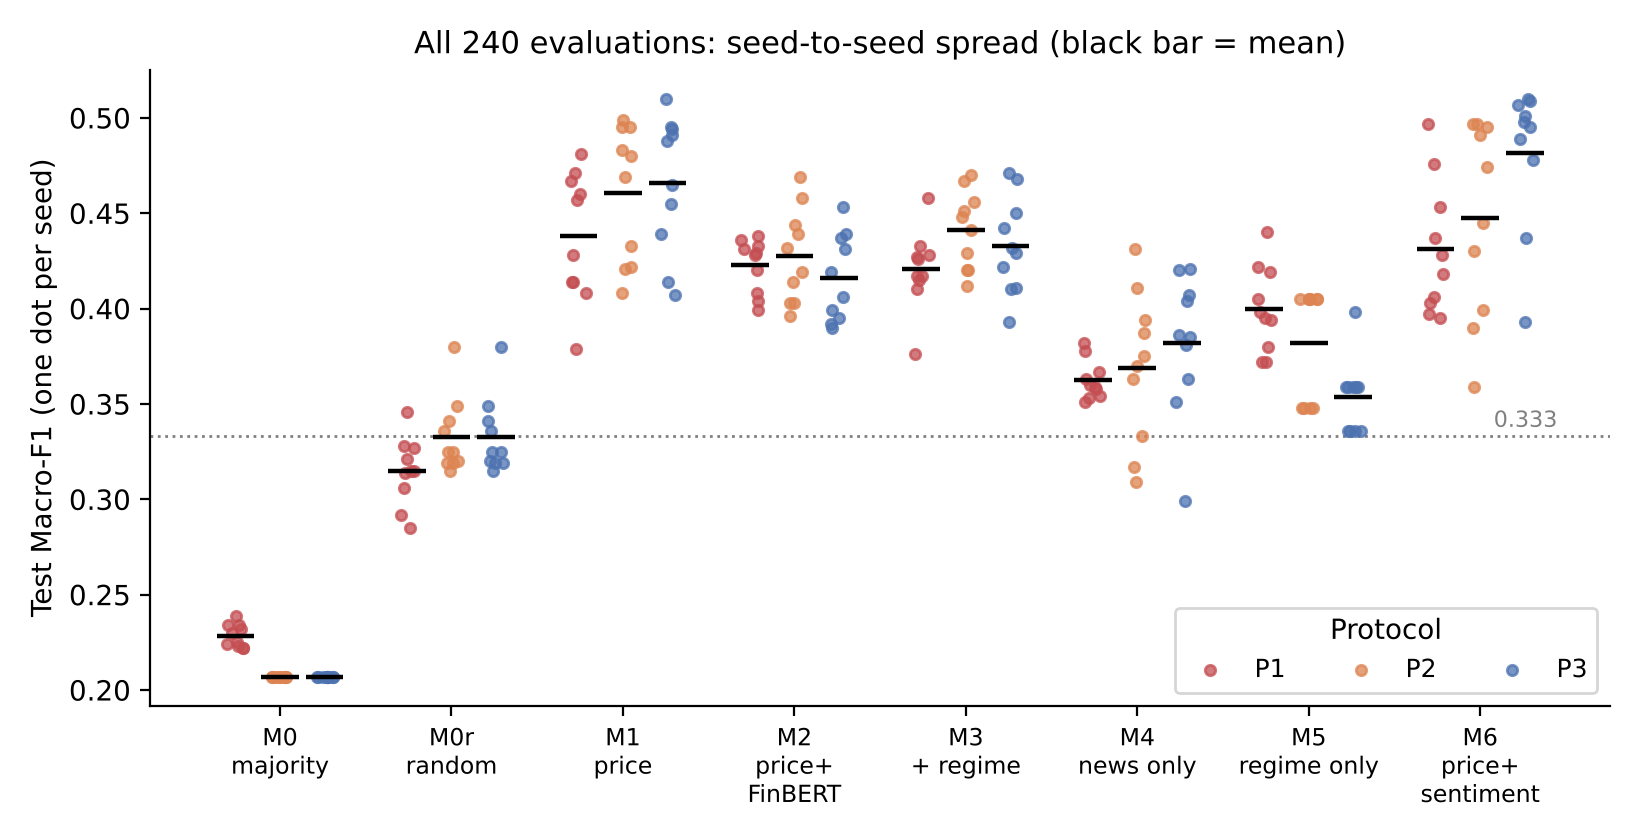
\includegraphics[width=\textwidth]{fig_seed_scatter.png}\caption[Test Macro-F1 of all 240 model--protocol--seed evaluations]{Test Macro-F1 of each of the 240 model--protocol--seed evaluations (one dot per seed; black bar: mean over seeds; dotted line: 0.333).}\label{fig:seeds}\end{figure}

For the models that use lagged prices and/or news (M1--M4) the looser protocols did \emph{not} score reliably higher than the strict one; all eight intervals for M1--M4 include zero. The exception is the regime-only model M5, which scores higher under both looser protocols (+0.046 and +0.028). Two mechanisms could contribute and were not separated here: under P1 a random split places near neighbours of each test day in the training set, and under P1 and P2 fitting the clusters on all data lets test-period structure shape the regime labels. P2$-$P3 shares the test rows and is the cleaner contrast (+0.028, interval near zero). For M6 the strict protocol scored \emph{higher} than the random split. This reversal reinforces that the protocol gaps are model-dependent; because P1 changes the test sample across seeds, the observed gap also reflects sample composition and run-to-run variability, not leakage alone. Hypothesis H1 is therefore \textbf{not supported in general}, and only weakly and exploratorily suggested for the model that relies solely on a slowly varying state.

\subsection{Value of News and Regime Information (RQ2)}\label{sec:regime-results}
\begin{table}[H]
\centering
\small
\begin{tabular}{lrccccc}
\toprule
Group & $n$ & Random & M1 & M2 & M3 & M6\\
 & & floor & price & +emb. & +emb.+reg. & +sent.\\
\midrule
All test & 317 & 0.333 & 0.466 & 0.416 & 0.433 & 0.482\\
Low-vol & 125 & 0.329 & 0.409 & 0.386 & 0.407 & 0.415\\
Mid-vol & 113 & 0.322 & 0.410 & 0.341 & 0.361 & 0.464\\
High-vol & 79 & 0.323 & 0.357 & 0.363 & 0.319 & 0.378\\
Stress window & 50 & 0.316 & 0.473 & 0.448 & 0.450 & 0.471\\
Outside stress & 267 & 0.334 & 0.451 & 0.391 & 0.416 & 0.467\\
\bottomrule
\end{tabular}
\caption[Test Macro-F1 by group under P3]{Test Macro-F1 by group under P3 (mean over ten seeds of the per-seed Macro-F1 on the group's rows). Group sizes are small, so group-level values are noisy.}\label{tab:levels}
\end{table}
\begin{table}[H]
\centering
\small
\begin{tabular}{lrccc}
\toprule
Group & $n$ & M2 $-$ M1 & M6 $-$ M1 & M3 $-$ M2\\
 & & (embedding) & (sentiment) & (regime input)\\
\midrule
All test & 317 & \textbf{$-0.050$ [$-0.087$, $-0.012$]} & $+0.016$ [$-0.017$, 0.049] & $+0.017$ [$-0.002$, 0.038]\\
Low-vol & 125 & $-0.023$ [$-0.079$, 0.031] & $+0.006$ [$-0.041$, 0.058] & $+0.021$ [$-0.002$, 0.043]\\
Mid-vol & 113 & $-0.069$ [$-0.147$, 0.003] & \textbf{$+0.054$ [0.004, 0.107]} & $+0.021$ [$-0.011$, 0.051]\\
High-vol & 79 & $+0.005$ [$-0.062$, 0.074] & $+0.020$ [$-0.041$, 0.081] & $-0.043$ [$-0.101$, 0.011]\\
Stress window & 50 & $-0.024$ [$-0.115$, 0.056] & $-0.001$ [$-0.079$, 0.072] & $+0.002$ [$-0.044$, 0.046]\\
Outside stress & 267 & \textbf{$-0.060$ [$-0.097$, $-0.017$]} & $+0.016$ [$-0.021$, 0.050] & \textbf{$+0.024$ [0.002, 0.047]}\\
\bottomrule
\end{tabular}
\caption[Differences in Macro-F1 between models, by group, with 95\% intervals]{Differences in Macro-F1 (second minus first model) with 95\% bootstrap intervals from resampling test rows. Bold: interval excludes zero. For news and regime together versus price only, M3 $-$ M1 is $-0.033$ [$-0.069$, 0.001] overall. Rows are resampled as if independent; temporal dependence is ignored, so intervals are probably too narrow.}\label{tab:diffs}
\end{table}
\begin{figure}[H]\centering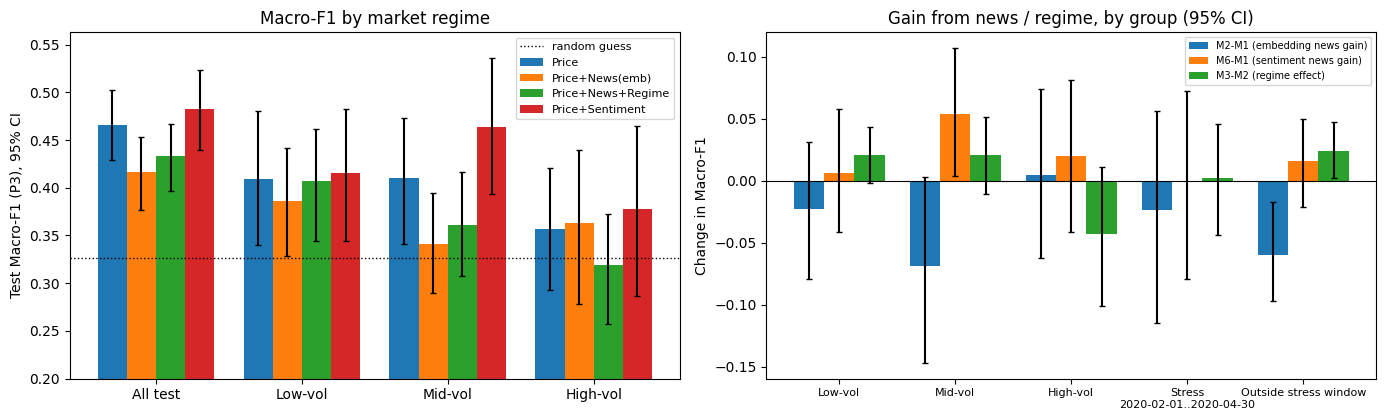
\includegraphics[width=\textwidth]{fig_regime_news_value.png}\caption[Macro-F1 and model differences by regime and stress window]{Test Macro-F1 (left) and model differences (right) by regime and stress window under P3, with 95\% row-bootstrap intervals; error bars are the intervals of Tables~\ref{tab:levels} and~\ref{tab:diffs}.}\end{figure}
Four findings follow.
\begin{enumerate}
\item \textbf{The FinBERT embedding hurts.} Adding it to the price model reduces Macro-F1 by 0.050 with an interval excluding zero; outside the stress window the reduction is 0.060.
\item \textbf{A low-capacity news input is about neutral.} Three sentiment scores give $+0.016$ overall with an interval including zero. The only interval excluding zero (Mid-vol, $+0.054$) is one of 24 comparisons and is treated as a hypothesis.
\item \textbf{The regime input adds little.} Adding the regime id to the price-plus-embedding model changes Macro-F1 by $+0.017$ (interval includes zero); the best news-plus-regime model (M3) does not beat price only. Outside the stress window the regime input gives $+0.024$ [0.002, 0.047], one of four intervals excluding zero (with M2$-$M1 overall and outside stress, and M6$-$M1 in Mid-vol); all four are treated as exploratory.
\item \textbf{No reliable extra news value detected in the stress window.} In 1 February--30 April 2020 no model with news information differs reliably from price only. With only 50 rows the intervals are wide (about $\pm0.05$ to $\pm0.09$), so moderate effects cannot be excluded.
\end{enumerate}

\subsection{The Stress Window}\label{sec:stress}
Within the stress window the price-only model reaches 0.473, the random floor 0.316, and the embedding and regime models 0.448 and 0.450. None of the news-related differences is reliably non-zero (Table~\ref{tab:diffs}). Mean FinBERT sentiment in March 2020 is $-0.319$ against $-0.176$ for the remainder of the test set, so the headlines do register the shock, but this did not translate into a measurable gain in next-day classification.

\subsection{Diagnostic: What the Models Predict}
Table~\ref{tab:classdiag} shows predicted class shares and per-class F1 for the price-only and sentiment models.
\begin{table}[H]
\centering
\begin{tabular}{lccc}
\toprule
 & Fall & Neutral & Rise\\
\midrule
True test share & 0.230 & 0.451 & 0.319\\
M1 predicted share & 0.191 & 0.545 & 0.263\\
M2 predicted share & 0.303 & 0.581 & 0.116\\
M3 predicted share & 0.302 & 0.525 & 0.173\\
M6 predicted share & 0.322 & 0.502 & 0.176\\
M1 per-class F1 & 0.291 & 0.687 & 0.420\\
M6 per-class F1 & 0.397 & 0.690 & 0.358\\
\bottomrule
\end{tabular}
\caption{Predicted shares and per-class F1 on the P3 test set (10 seeds).}\label{tab:classdiag}
\end{table}
The Neutral-class F1 is almost identical for M1 and M6 (0.687 and 0.690). The sentiment model trades Rise for Fall (Fall F1 $0.291\to0.397$, Rise F1 $0.420\to0.358$) and predicts Fall on 32\% of days versus 19\% for the price-only model (true share 23\%). This is consistent with the small and unreliable overall change: the news input shifts the balance between the two directional classes but adds no clear skill.

Figure~\ref{fig:shares} shows the predicted shares of Table~\ref{tab:classdiag} against the true shares. All four models predict Neutral more often than its true share (0.451), and the models that use news predict Rise for only 12--18\% of rows against a true share of 32\%, so a large part of the differences in Macro-F1 between models reflects how the predictions are distributed across classes.
\begin{figure}[H]\centering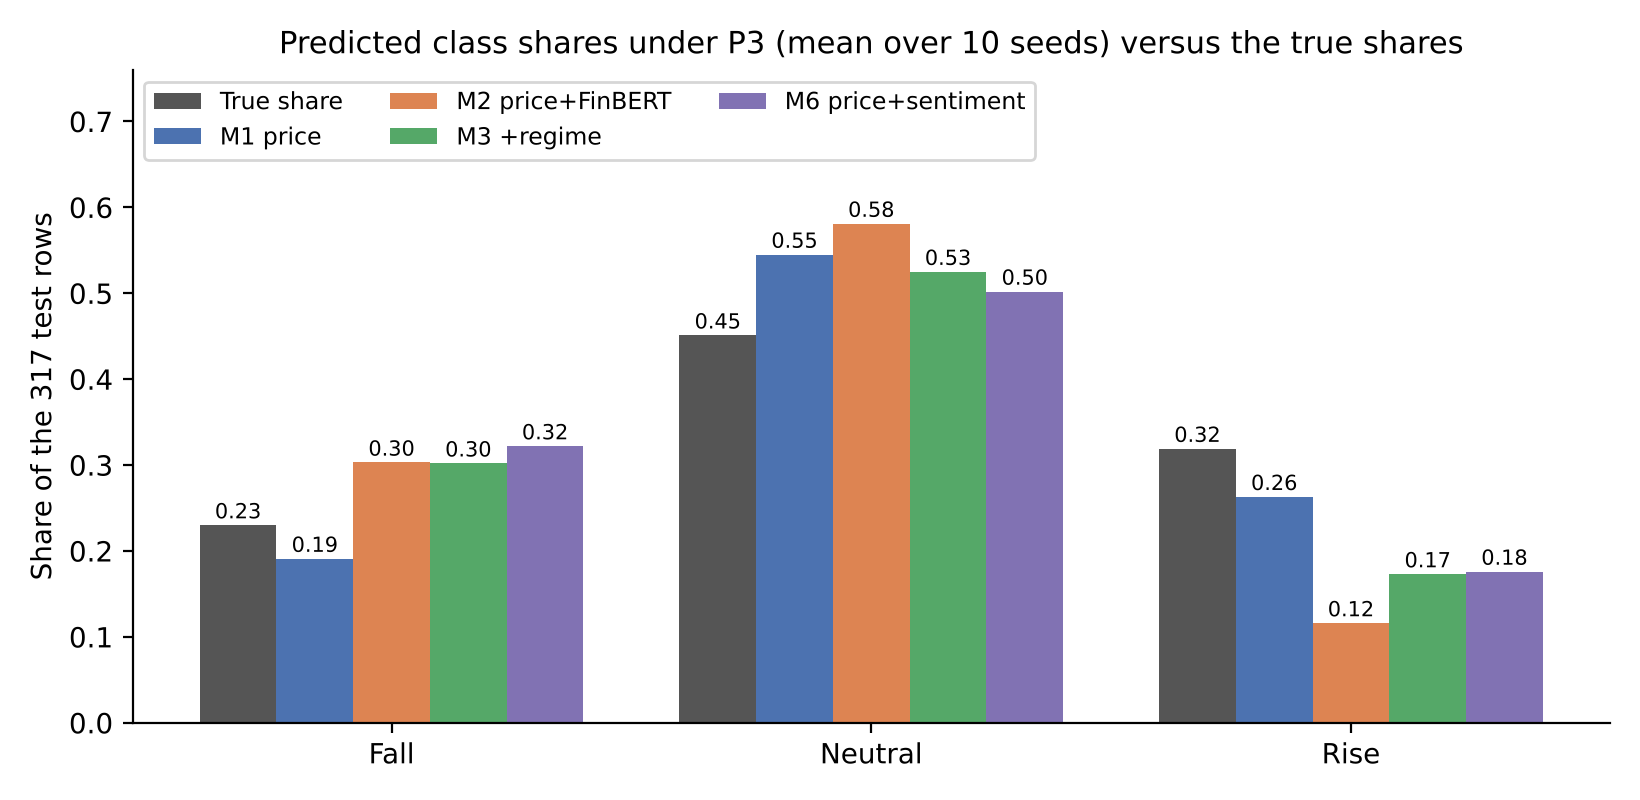
\includegraphics[width=\textwidth]{fig_class_shares.png}\caption[Predicted and true class shares on the P3 test set]{Predicted class shares on the P3 test set (mean over ten seeds) for the price-only, price-plus-embedding, price-plus-embedding-plus-regime and price-plus-sentiment models, against the true shares.}\label{fig:shares}\end{figure}

\subsection{Summary of Hypotheses}
\begin{table}[H]
\centering
\begin{tabular}{p{5.2cm}p{9.3cm}}
\toprule
Hypothesis & Outcome\\
\midrule
H1: looser protocols overstate performance & Not supported in general; weak, exploratory evidence for the regime-only model (M5), with sample composition not separated from leakage.\\
H2: the value of news differs across regimes & Not supported for embeddings (no gain in any regime). For sentiment a gain appears only in Mid-vol and is not robust; insufficient evidence of regime dependence.\\
H3: an explicit regime input improves the multimodal model & Not supported ($+0.017$, interval includes zero; M3 does not beat M1). One interval outside the stress window ($+0.024$) excludes zero and is exploratory.\\
\bottomrule
\end{tabular}
\caption{Outcome of the hypotheses.}
\end{table}

\newpage
\section{Discussion and Limitations}\label{ch:discussion}
\subsection{What the Models Learn}
All learned models exceed the mean Macro-F1 of the uniform-random baseline, but this does not imply that every model is reliably better in a statistical sense. Label distributions vary across regimes: the Neutral share is 64.2\% in Low-vol, 54.9\% in Mid-vol and 28.8\% in High-vol across the full set of rows. This is an association between recent market conditions and the next-day class distribution; it does not establish that most predictive skill comes from forecasting volatility magnitude rather than direction. The price-only model is already competitive, and adding a regime label to the price-plus-embedding model does not produce a reliable overall improvement.

\subsection{Why the Embedding Hurts}
The 768-dimensional embedding must be mapped to a useful representation from about 1{,}460 training rows. The train--test gaps in Table~\ref{tab:overfit} (0.138 for M2, 0.319 for M4, against 0.011 for M1) are the signature of overfitting, and the significant decrease when the embedding is added to the price model is consistent with it. Two further factors may contribute. First, the daily mean-pooled embedding varies little from one day to the next (cosine similarity 0.963 between consecutive days and 0.951 between random days), so the useful contrast is small relative to the 768 dimensions. Second, the headline supply and tone change across the decade (49 headlines per day in training versus 26 in test after capping; mean sentiment $-0.068$ versus $-0.184$), so a high-capacity news model can learn era-specific patterns that do not transfer. This report did not test these explanations separately; they are hypotheses consistent with the data.

\subsection{Why Protocol Effects Are Small}
The regime-only model scores higher under both looser protocols, consistent with a slowly varying regime assignment being sensitive to random splitting and to fitting clusters on the full sample. However, P1 uses a different random test set for each seed, while P2/P3 use the chronological test set. Consequently, the protocol gaps combine protocol changes with test-sample composition and run variability; they do not isolate a causal effect of leakage. These results apply only to the specific split and preprocessing changes examined here. They do not rule out other forms of leakage, including use of information unavailable at prediction time.

\subsection{The Stress Window}
News did not add reliable value during the February--April 2020 episode in this data, although headline sentiment clearly moved. With 50 test rows the analysis has low power, so the result is best read as ``no large effect detected'' and not as ``no effect''. Because this study uses one benchmark, a small stress subset and date-only headlines, it cannot settle whether news is generally more valuable during volatile markets. Differences in assets, label construction, data timing and evaluation protocols prevent direct comparison with published point estimates.

\subsection{Limitations}
\begin{itemize}
\item One asset (SPY), one benchmark and one decade; results may not transfer to other markets.
\item Only 317 test rows (125, 113 and 79 by regime; 50 in the stress window): intervals are wide and small effects cannot be detected. Test rows are overlapping, autocorrelated daily observations, so bootstrap intervals that treat them as independent are probably somewhat too narrow.
\item Headlines carry a date but no publication time. A headline dated $t$ precedes the predicted move only if it was published by the close of day $t$; this could not be verified.
\item Headline volume and tone differ across the three periods, so train and test distributions differ.
\item Regimes are data-driven clusters (three clusters on rolling 20-day return and log-volatility), not validated economic states; the Mid-vol and High-vol regimes switch frequently (median run length 4 days).
\item The three protocols were evaluated on different test samples (P1 uses a random test set), so protocol gaps combine leakage and sampling differences.
\item About 24 comparisons were examined; isolated significant intervals are hypotheses. M6 and the random-guess baseline were added after seeing pilot results (Appendix~\ref{app:transparency}).
\item Fifteen expected trading days are missing from the recovered daily series and were not interpolated.
\item No transaction costs, trading rule or profitability analysis is attempted, and no causal claim is made.
\end{itemize}

\newpage
\section{Conclusion and Future Work}\label{ch:conclusion}
On the NIFTY benchmark, with strict chronological evaluation, a small price-only LSTM was the model to beat. FinBERT embeddings of daily headlines reduced out-of-sample Macro-F1; a low-dimensional sentiment summary gave at most a small and statistically unreliable gain; and an explicit market-regime input added little because the price window already encodes recent volatility. No evidence was found that news is more valuable during the 2020 stress period, although the sample is small. Moving from a strict to a looser evaluation protocol did not systematically inflate results, except for a model relying solely on a persistent regime label.

\begin{keybox}
\textbf{Take-aways.}
(i) Evaluate against a strong price-only baseline and a random-guess floor; a majority baseline is a misleading Macro-F1 floor.
(ii) Fit all preprocessing and regimes on training data only.
(iii) Expect high-dimensional text embeddings to overfit small samples, and prefer compact summaries or stronger regularisation.
(iv) Report every model and comparison run, and treat isolated significant intervals as hypotheses.
\end{keybox}
\subsection{Future Work}
\begin{itemize}
\item \textbf{Gated fusion (M7).} A regime-conditioned gate between the price and news embeddings is implemented but not evaluated; it would test whether news can be made useful conditionally.
\item \textbf{Lagged window ($\mathrm{LAG}=1$).} Re-running the pipeline with windows ending one day earlier, as in the benchmark's own prompt, would show how sensitive the conclusions are to the timing convention.
\item \textbf{Stronger regularisation of the news branch,} e.g.\ low-rank projections, PCA, or weight decay and dropout search on validation data only.
\item \textbf{More assets and periods,} and a block bootstrap that respects autocorrelation.
\item \textbf{Publication-time stamps for headlines} to remove the main timing uncertainty.
\end{itemize}

\newpage
\appendix
\section{Transparency Statement}\label{app:transparency}
\begin{itemize}
\item The primary models (M0--M5) and the three protocols were specified before running the experiments. The random-guess baseline M0r and the sentiment model M6 were added after a pilot run showed that the news-only and price-plus-embedding models overfit; results for both are reported regardless of outcome.
\item The number of seeds was increased from 3 to 10 after observing that seed-to-seed variation was as large as the effects of interest. In the 3-seed pilot, M6 appeared stronger (about 0.503); with 10 seeds the value was 0.482 and the difference to M1 was not significant, so the 10-seed result is the one reported. No hyper-parameters were changed.
\item Price inputs were converted to scale-free features before any model was run, because raw price levels drift over the sample.
\item Up to 50 headlines per day were sampled at random (fixed seed) to bound compute and reduce volume differences across periods.
\item Fifteen early rows without 20 days of history were excluded so that all models use the same samples.
\item The label alignment (next-trading-day close-to-close return) was verified empirically on 2{,}110 rows.
\item About 24 pairwise comparisons were examined (4 comparisons $\times$ 6 groups).
\item M7 and the $\mathrm{LAG}=1$ option exist in the code but were not run on real data.
\item \textbf{Use of tools.} AI-based assistants were used during the project for planning, code drafting and wording suggestions. All experiments were run by the author, and the reported numbers are those produced by the executed notebook.
\end{itemize}

\section{Reproducibility}
The code, executed notebook, raw cell outputs and figure-generating scripts are in the project repository
(\texttt{github.com/Hamza-Faarooq/btp-regime-aware-multimodal-forecasting}). The reported results were produced by the executed Google Colab notebook and its saved outputs. The repository also contains modular scripts for data preparation, regime assignment, FinBERT encoding, model training and analysis. The full 270-run script grid includes M7, but M7 was not evaluated on real data for the reported results; the reported real-data grid covers M0--M6 across three protocols and ten seeds. Random seeds are fixed for model initialisation (0--9), headline sampling (1234), $k$-means (0), and the bootstrap analysis. The modular command-line path was tested on a synthetic mock dataset; a clean end-to-end reproduction from raw data has not yet been independently verified.

\section*{List of Important Symbols}
\addcontentsline{toc}{section}{List of Important Symbols}
\begin{itemize}
\item $t$ - Date of a dataset row; the label concerns the move from $t$ to the next trading day
\item $y_t\in\{\text{Fall},\text{Neutral},\text{Rise}\}$ - Class label
\item $X_t\in\mathbb{R}^{10\times 12}$ - Price-feature window ending at $t$
\item $n_t$ - News representation of day $t$ (768-d embedding or 3 sentiment scores)
\item $g_t$ - Volatility regime of day $t$ (Low-, Mid-, High-vol)
\item $\mathrm{ret}_{20}$, $\sigma_{20}$ - 20-day return and 20-day standard deviation of daily returns
\item $\Fone$ - Harmonic mean of precision and recall; Macro-$\Fone$ is its mean over classes
\item P1, P2, P3 - Evaluation protocols (random, chronological, strict chronological)
\item M0--M7 - Models (Table~\ref{tab:models}; M7 is implemented but not evaluated)
\item $z_{\text{price}}, z_{\text{news}}, e_{\text{regime}}$ - Branch embeddings of the network
\item $\mathrm{LAG}$ - Offset between the label date and the last day of the price window
\end{itemize}

\begin{thebibliography}{99}\addcontentsline{toc}{section}{References}
\bibitem{araci2019} \textbf{Araci, D.} (2019). \emph{FinBERT: Financial Sentiment Analysis with Pre-trained Language Models}. arXiv:1908.10063.
\bibitem{bailey2014} \textbf{Bailey, D. H., Borwein, J. M., Lopez de Prado, M., \& Zhu, Q. J.} (2014). Pseudo-Mathematics and Financial Charlatanism: The Effects of Backtest Overfitting on Out-of-Sample Performance. \emph{Notices of the American Mathematical Society}, 61(5), 458--471.
\bibitem{bailey2015} \textbf{Bailey, D. H., Borwein, J. M., Lopez de Prado, M., \& Zhu, Q. J.} (2015). The Probability of Backtest Overfitting. \emph{Journal of Computational Finance}. SSRN 2326253.
\bibitem{gu2024} \textbf{Gu, W., et al.} (2024). \emph{Predicting Stock Prices with FinBERT-LSTM: Integrating News Sentiment Analysis}. arXiv:2407.16150.
\bibitem{halder2022} \textbf{Halder, S.} (2022). \emph{FinBERT-LSTM: Deep Learning based Stock Price Prediction using News Sentiment Analysis}. arXiv:2211.07392.
\bibitem{hochreiter1997} \textbf{Hochreiter, S., \& Schmidhuber, J.} (1997). Long Short-Term Memory. \emph{Neural Computation}, 9(8), 1735--1780.
\bibitem{karadas2025} \textbf{Karada\c{s}, E., Eravci, B., \& Ozbayoglu, A. M.} (2025). \emph{Multimodal Stock Price Prediction}. arXiv:2502.05186.
\bibitem{kraus2017} \textbf{Kraus, M., \& Feuerriegel, S.} (2017). Decision support from financial disclosures with deep neural networks and transfer learning. \emph{Decision Support Systems}, 104, 38--48. arXiv:1710.03954.
\bibitem{saqur2024} \textbf{Saqur, R., Kato, K., Vinden, N., \& Rudzicz, F.} (2024). \emph{NIFTY Financial News Headlines Dataset}. arXiv:2405.09747.
\bibitem{wang2026} \textbf{Wang et al.} (2026). FusionLSTM-CNF: a confidence-calibrated multi-modal late fusion framework for robust stock movement prediction under uncertainty. \emph{Scientific Reports}, 16, 17494. doi:10.1038/s41598-026-43381-3.
\bibitem{zong2024} \textbf{Zong et al.} (2024). \emph{Stock Movement Prediction with Multimodal Stable Fusion via Gated Cross-Attention Mechanism}. arXiv:2406.06594.
\end{thebibliography}

\end{document}
